\section{Experimental Setup}
Query expansion using pseudo relevance turns out to yield better results in terms of relevance compared to a TF/IDF search,
which is the common approach in today's search engines.
Even though query expansion delivers more relevant search results,
the results have to be available fast enough to be used in interactive environments.
In other words, the results have to be available within 100 ms.
Both implementations will be evaluated against a baseline search.
The baseline search will in both cases be a multi term search.

Query expansion requires the search engine to process an initial query,
and is then sending a new query to retrieve the final result.
As the search requires two searches,
the query expansion implementation will naturally yield higher response times.
The most interesting results are how much slower the query expansion is compared to the baseline search.

\subsection{Data Set}
\label{sec:dataset}
Both experiments use the data set described in this section.
The data set consits of photo data gathered from the Flickr API\footnote{\url{https://www.flickr.com/services/api/}}.
Flickr was chosen as the data source as tags have been found to provide strong data for query expansion \cite{ir-hashtag}.
All the photos were retrieved using Flickr's endpoint for fetching the last published photos.
However, the API limits the number of requests per hour.
The photos were gathered over a period of about three months, March 2017 to the end of May 2017.
The data set used in the experiment consists of 4,561,816 photos and 9,993,411 tags.
Of all the photos, a total of 1,708,324 photos have 1 or more tags,
which means that 37 \% of the photos have tags.
Counting all the photos with at least one tag,
each photo has 5.8 tags in average.
Every tag is user created by the person who posted the photo.
Flickr also has an analyzer which ads additional tags,
but these tags are not available through the API.

The pie chart in figure \ref{fig:pie-chart-tag-distribution} shows the number of tags on each photo,
and the chart shows that photos with 5 tags are the largest group.
Most of the photos have multiple tags,
which improves the tag generation.
If the top-k documents only have one of the same tag,
the algorithm will not generate additional tags.
As a result, more tags results in better data for the query expansion algorithm.

\begin{figure}[h!]
  \centering 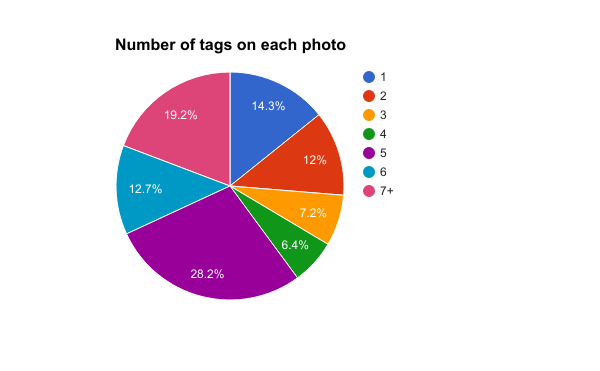
\includegraphics[width=1\linewidth]{img/number-of-tags-distribution.png}
  \caption{Pie chart that shows the distribution on how many tags each photo have.}
  \label{fig:pie-chart-tag-distribution}
\end{figure}

\subsection{Lucene Experiment}
All the data types indexed in the Lucene experiment can be seen in table \ref{tbl:lucene-field-types}.
Even though only the tag fields are used in the algorithm,
more fields are indexed to make the experiment closer to a real world application.
\texttt{StringField} will be indexed as a single token,
which is useful for aggregating or filtering on the field.
\texttt{TextField} is indexed for full-text search.
With the full-text search indexing the field also stores the term frequencies,
which is required for the query expansion algorithm.
The reason for using \texttt{LongPoint} on a date is to make it efficient to range searches.

\begin{table}[h!]
    \begin{tabular}{|l|l|}
    \hline
    \textbf{Field} & \textbf{Type}      \\ \hline
    id           & StringField          \\ \hline
    title        & TextField            \\ \hline
    description  & TextField            \\ \hline
    dateuploaded & LongPoint            \\ \hline
    urls         & Array of StringField \\ \hline
    tags         & Array of TextField   \\ \hline
    \end{tabular}
    \centering
    \caption{Field types of every field used in the experiment.}
    \label{tbl:lucene-field-types}
\end{table}

A different performance metric is used for the Lucene experiment,
as Lucene is a Java library and is not a complete framework with a REST API compared to Elasticsearch.
The Lucene implementation is evaluated by measuring the time from the query is sent to index until the result is retrieved.
This is not a real world experiment setup,
but this evaluation is used to reveal how much slower the query expansion algorithm is compared to the baseline query.
To retrieve an accurate measurement a Java method called \texttt{System.nanoTime()} is used.
\texttt{System.nanoTime()} is the most precise method available in Java to measure elapsed time.

\subsection{Elasticsearch Experiment}
Most web applications today with a search field will have a web server and a search engine on the backend.
Figure \ref{fig:elasticsearch-experiment-setup} displays a common setup for web application with search capabilities.
The client sends a search to the web server which process the request and sends it to the search engine.
After finding the most relevant documents, the result is sent back from the search engine to the web server,
which again sends the result to the user.
As mentioned earlier,
the requirement for interactive applications are that no operation takes longer than 100 ms.
Response time is measured from the request is sent from the client to the response arrives at the client.
To verify that the query expansion plugin for Elasticsearch is fast enough to meet the interactive requirements,
the experiment was setup as shown in figure \ref{fig:elasticsearch-experiment-setup}.
The client on the figure was the author's laptop,
and the backend was setup to mimic a real world environment.
The backend consists of two main components, a web server and a search engine.

\begin{figure}[h!]
  \centering 
\includegraphics[width=0.9\linewidth]{img/elasticsearch-experiment-setup.png}
  \caption{Overview of the Elasticsearch experiment setup.}
  \label{fig:elasticsearch-experiment-setup}
\end{figure}

As web applications often use cloud providers, the tests also needed to be conducted using cloud providers.
The requirement set for the cloud provider was: need to be widely used, have servers in Europe and provide VPS services.
Possible providers were: Amozon Web Services\footnote{\url{https://aws.amazon.com/}},
Google Cloud Platform\footnote{\url{https://cloud.google.com/}} and Digital Ocean\footnote{\url{https://www.digitalocean.com/}}.
Google Cloud Platform was chosen as the service provider, as you have more flexibility to choose between number of cores and the memory size and
the author had knowledge of the platform.
Tests were conducted using two Google Compute Engine instances.
Web services always strive to place the servers as close to the users as possible.
To make the experiment simulate a real world scenario both the instances were placed in the reagion called \textit{europe-west1-c}.

\subsubsection{Elasticsearch Instance}
The instance running Elasticsearch had the following specifications: 2 vCPUs, 10 GB memory and 20 GB SSD.
Elasticsearch's documentation\footnote{\url{https://www.elastic.co/guide/en/elasticsearch/guide/current/hardware.html}}
suggests that memory will be the most important resource in most use cases.
As a result more memory was chosen over the number of CPUs.
An important setting in Elasticsearch is the heap size.
By default the heap memory size is set to 1 GB,
but was changed to 5 GB in the test environment.
A logical assumption would be to set the Elasticsearch to use all the available memory, except the memory needed for the operating system.
However, Elasticsearch's underlying structure Lucene also needs memory.
Lucene stores the data in separate files.
The data structure inside the files is immutable, which makes them optimized for caching.
With this strategy Lucene optimizes the underlying operating system's eager to hold small and often used files in memory.
According to the Elasticsearch documentation\footnote{\url{https://www.elastic.co/guide/en/elasticsearch/guide/current/heap-sizing.html}},
the heap size should be set to 50\% or less, of the available memory.

Most operating systems today also comes with swapping turned on by default.
If the operating system decides to swap, it would significantly reduce the performance.
To avoid the problem, swapping was turned off on the Elasticsearch instance.

\subsubsection{NodeJS Instance}
The instance running NodeJS had the following specifications: 4 vCPUs, 4 GB memory and 10 GB SSD.
On the web server we want to be able to handle as many requests as possible.
The number of requests the server is able to handle are closely linked to the number of cores.
That is why the Node.js instance has more cores at the cost of less memory.

Node.js is by design single threaded, which would make 3 of the cores on the Node.js server being idle.
However, this problem can be solved by using tool called pm2\footnote{\url{http://pm2.keymetrics.io/}}.
pm2 has a feature called \textit{cluster mode}, which may spawn multiple Node.js instances.
To allow maximum CPU utilization, pm2 can be configured to spawn as many Node.js instances as the number of cores.

To test the implementation the Node.js web server implemented two different endpoints.
One endpoint is used to test the query expansion plugin,
and the other is used to test a multi term query.

\subsubsection{Performance Metrics}
Evaluating the Elasticsearch plugin is done by measuring the response time from a client sends the request to the response arrives.
The response time can be broken down into two separate parts: latency and execution, as shown in figure \ref{fig:latency-measurements}.
In this thesis latency, is defined as the time it takes for a signal to go from the client to the web server and back.
Execution time is defined from the web server recieves a request from the client, until the web server sends a response back to the client.
This means that the execution time also includes the processing time on the search engine.


\begin{figure}[h!]
  \centering 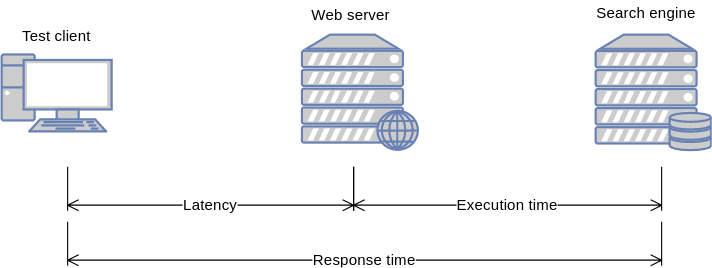
\includegraphics[width=0.9\linewidth]{img/latency-measurements.png}
  \caption{Overview of the different measurements used when evaluating the implementation.}
  \label{fig:latency-measurements}
\end{figure}
